\documentclass[14pt]{report}
\usepackage[spanish]{babel}
\usepackage[utf8]{inputenc}
\usepackage{amsmath}
\usepackage{graphicx}
\pagestyle{plain}

\title{Interpolación Lagrange}
\author{Nieves García \ Javier Contreras \ Kevin Cabrera}
\date{12 de Mayo de 2013}

\begin{document}

\maketitle

\pagebreak
\pagebreak
\begin{abstract}
 El teorema del valor medio o de los incrementos finitos de Lagrange, es uno de los teoremas más importantes  
 del análisis matemático, no por sus aplicaciones prácticas, si no por la capacidad que ofrece para la
 demostración de otros grandes teoremas.\
 En este documento se tratará este teorema desde un punto práctico, y se estudiará su comportamiento en un tipo de función.
 Además se implementará en lenguaje de programación, en este caso Python, en el que estudiaremos sus pros y sus contras. 
\end{abstract}

\newpage
\tableofcontents
\pagebreak

\chapter{Motivación y objetivos}
Se ha elegido el teorema de Lagrange para este estudio principalmente por su facilidad ante la tarea de encontrar puntos vaticinados en dicho teorema,
y sencillez en su implementación Python.
\section{Python y Latex}
Python es un lenguaje de programación interpretado, uno de las principales opciones para la realización de textos científicos. Ante la necesidad de familiarizarse tanto 
con este tipo de escritura, como el lenguaje de programación , se ha realizado un estudio del teorema elegido y su implementación en Python, plasmando así los resultados obtenidos en este documento. 
que se utilizará como herramienta para la realización de la tarea.
Se tiene por lo tanto como principal finalidad familiarizarse con el lenguaje de programación, que muchas veces resulta complicado para el que no esté acostumbrado a tratarlo, además
de la creación de informes científicos, en este caso haciendo uso de \LaTeX.
\section{Objetivos secundarios}
Se observarán además otros puntos de la implementación en Python:
\begin{itemize}
\item Posibilidades que ofrece programación en lenguaje Python.
\item Calidad de documentos realizados en \LaTeX.
\item Ampliar mayor conocimiento tanto en lenguaje científico,programación y en el Teorema de Lagrange.
\end{itemize}
\pagebreak

\chapter{Fundamentos Teóricos}
El teorema de Lagrangem, también conocido como teoría del punto medio o teorema de los incrementos finitos, es una propiedad de las funciones derivables en un intervalo.
Tiene un fin más teórico que práctico, pero no por ello deja de ser una de las bases que fundamenta gran parte del cálculo matemático.
\section{El teorema}
Pese a su pobre capacidad de aplicación a problemas prácticos en matemáticas, física. Esta vez, se estudiará de una forma relativamente práctica, sin aundar demasiado en su definición teórica.
Veamos su definición formal:
Sea $ f $una función definida en un intervalo $ [a,b] $, y derivable en $ (a,b) $. Existe un punto $ c $ perteneciente al intervalo $ (a,b) $ de forma que: \\
\[ f(c)=\frac{f(b) - f(a)}{b - a} \]

\section{Fase de cálculo}

Sea $ f(x)=ln(6x) $ estudiemos los puntos vaticinados en el teorema de Lagrange para un intervalo $ (1,7) $. Se sabe que, en virtud del teorema, 
\[f'(c)= \frac{f(7)-f(1)}{7-1} \] esto es: \[ f'(c) = \frac{ln(6*7)-ln(6)}{6} \] Por las propiedades de los logaritmos, se obtiene:
\[f'(c)= \frac{ln(7)}{6} \]
Por otra parte, se tiene que la derivada de $ f(x)= ln(6x) $ es $ \frac{6}{6x} = \frac{1}{x} $. Tomando $ x=c $ :
\[ \frac{1}{x} = \frac{ln(7)}{6} \] 
Despejando la c: $ c= \frac{6}{ln(7)} $ Que equivale apróximadamente: $ c = 4.32808512267 $ .Que es el resultado que se obtendrá tras la implementación del programa
en Python.

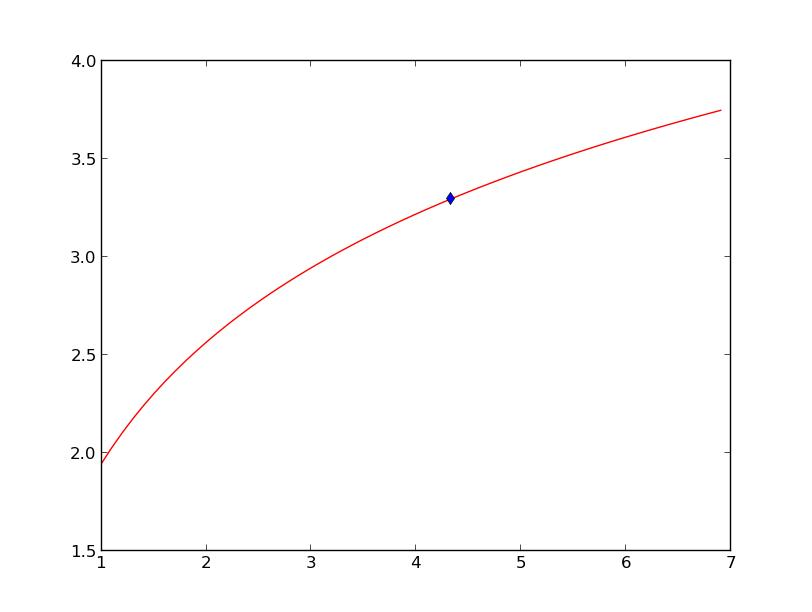
\includegraphics[scale=0.55]{graficofinal.jpeg}

\pagebreak


\chapter{Procedimiento experimental}
En este apartado se tratarán los pasos seguidos para la realización del experimento en lenguaje de programación, los materiales utilizados, y los resultados obtenidos.
\section{Descripción de los experimentos}
Se ha implementado el programa Lagrange de forma que una vez se pase por el intérprete, enuncie por pantalla el teorema a tratar y la función por la que esta preparada para estudiar.
En un pricipio pedirá por pantalla dos elementos flotantes, los cuales se corresponden con en intervalo abierto $ (a,b) $. \\
A continuación se realiza una llamada a una subfunción que contiene la fórmula del logaritmo neperiano, y se continuará con el proceso del punto, además de imprimir por pantalla una grafica de dicha función. 
\section{Resultados obtenidos}
Tras la ejecución de todo el programa, para un intervalo $ (1,7) $ obtenemos un punto $ c = $ que representa el único punto de la función que respeta que la recta tangente en dicho punto, 
tiene la misma pendiente que la recta secante que une los puntos $ (a,f(a)) $ y $ (b,f(b)) $ . Dicho punto se obtiene con una precisión mayor a $ 10^{-9} u $ , pero truncada en la doceava décima.\\
Para situaciones prácticas puede resultar un resultado más que fiable, sin embargo, respecto al apartado teórico se puede precisar mucho más, de hecho, el resultado real es $ \frac{ln(7)}{6} $. \\
Ante la falta de capacidad de la obtención de resultados mas simbólicos que reales, como el de casi todos los puntos de funciones trascendentales, supone una cierta limitación para el programa.
Esto es así ya el computador no tiene infinita memoria, por lo que no puede dar infinitas cifras decimales. 
\section{Análisis de los resultados}
El punto c obtenido, obviando su truncamiento, es único, y varía en cuanto a la proporción que se tome el intervalo. Estos puntos siempre seran dados con un cierto error de truncamiento, que se compensa 
frente a la rapidez del programa.\\
Resultará en este ejemplo no muy práctico la velocidad con la que se ejecute el programa, pero si lo puede llegar a ser para códigos similares, o con otros fines que, una persona tardarìa varios minutos en resolver el problema.

\pagebreak

\chapter{Conclusiones}
Durante todo el proceso de estudio, se ha concluido que
\begin{itemize}
          
  \item Velocidad: El lenguaje de programación Python, ha sido útil en este experimento, ya que ofrece una mayor rapidez a la hora de realizar calculos medianamente laboriosos y ha permitido una elaboración del programa de forma concisa y clara,
         Python, pese a que puede resultar dificil de comprender para aquel que no tiene conocimiento de computación, en este caso a sido relativamente sencillo crear dicho programa, por lo que es una buena opción ante cualquier necesidad de cálculo
  \item Ventajas: Los documentos realizados en \LaTeX ofrecen una posiblidad mucho más amplias que un procesador de texto corriente, ya que puedes,
         personalizar tanto la apariencia como escribir con lenguaje matemático
  \item Conocimiento: Ante la necesidad de ajustarse a las nuevas tecnologías, la realización de textos científicos es un ítem fundamental par acualquier estudiante de ciencias. Gracias a este trabajo, se ha conseguido unir los conocimientos 
         matemáticos con la programación, y el uso de procesadores como \LaTeX
          

\end{itemize}
\pagebreak
\chapter{Bibliografía}

\begin{itemize}
 \item http://es.scribd.com/doc/53052350/47/Tablas-de-simbolos-matematicos-frecuentes
 \item http://es.wikipedia.org/wiki/LaTeX
\end{itemize}


\pagebreak




\end{document}